\chapter{Конструкторская часть}

Ниже приведены схемы алгоритмов, упомянутых в аналитической части.
\section{Поиск расстояния Левенштейна}
Ниже приведены схемы различных реализаций алгоритма поиска расстояния Левенштейна:
\begin{itemize}
	\item рисунок~\ref{fig:lev_rec} - схема рекурсивной реализации;
	\item рисунок~\ref{fig:lev_rec_mem} - схема рекурсивной реализации с мемоизацией;
	\item рисунок~\ref{fig:lev_iter} - схема итеративной реализации.
\end{itemize}
\subsection{Рекурсивная реализация }
\begin{figure}[H]
	\centering
	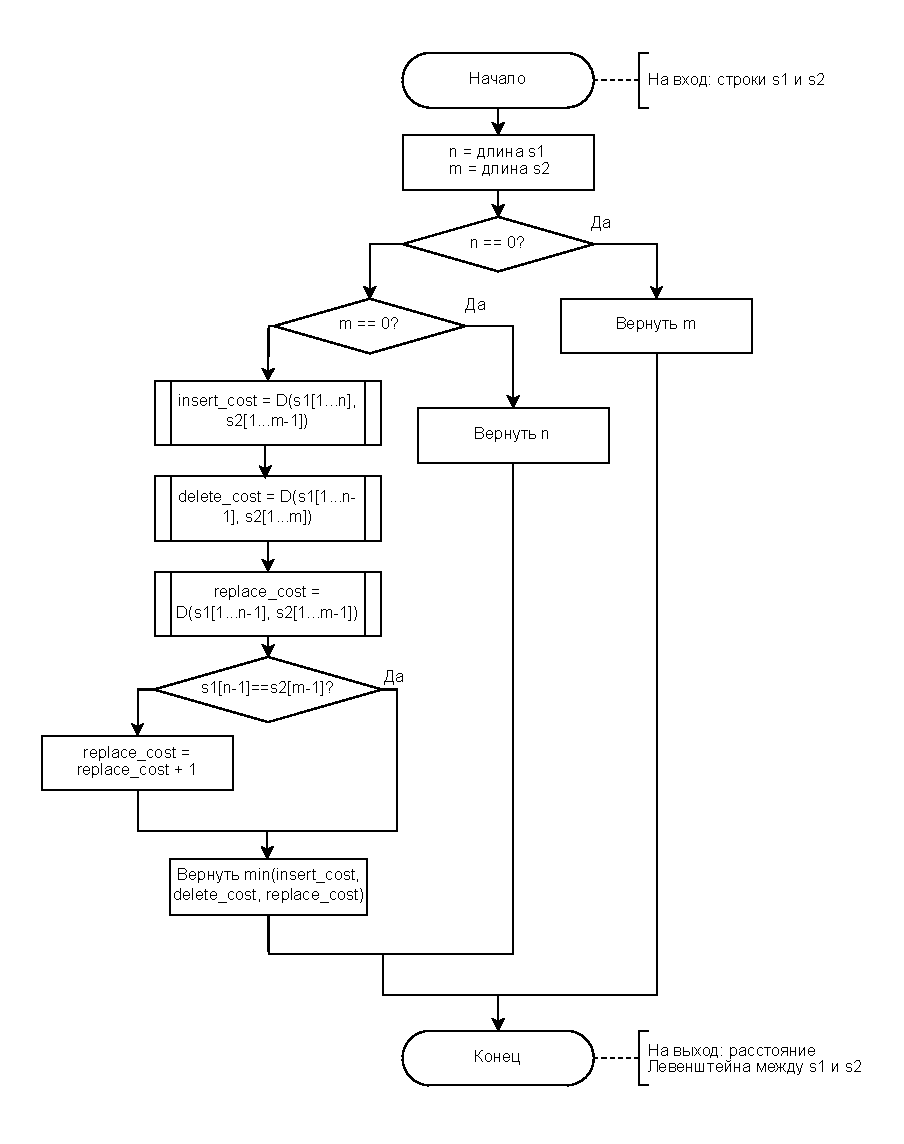
\includegraphics[width=0.8\textwidth]{levenstein_recursion.pdf}
	\caption{Схема рекурсивной реализации алгоритма поиска расстояния Левенштейна}
	\label{fig:lev_rec}
\end{figure}
\subsection{Рекурсивная реализация с мемоизацией}
\begin{figure}[H]
	\centering
	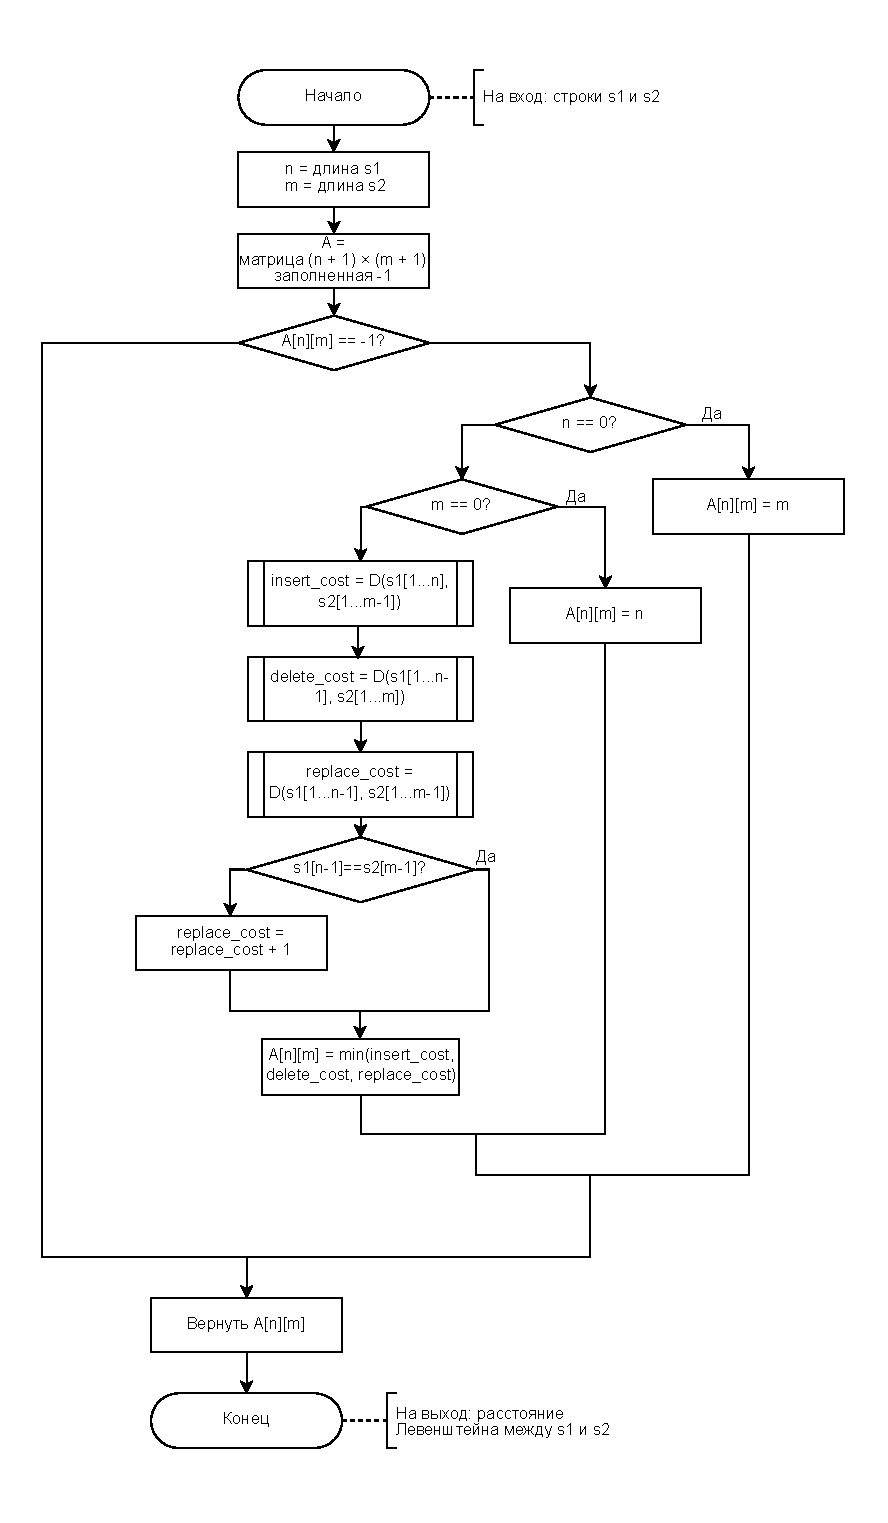
\includegraphics[width=0.7\textwidth]{lev_rec_mem.pdf}
	\caption{Схема рекурсивной реализации алгоритма поиска расстояния Левенштейна с мемоизацией}
	\label{fig:lev_rec_mem}
\end{figure}
\subsection{Нерекурсивная реализация }
\begin{figure}[H]
	\centering
	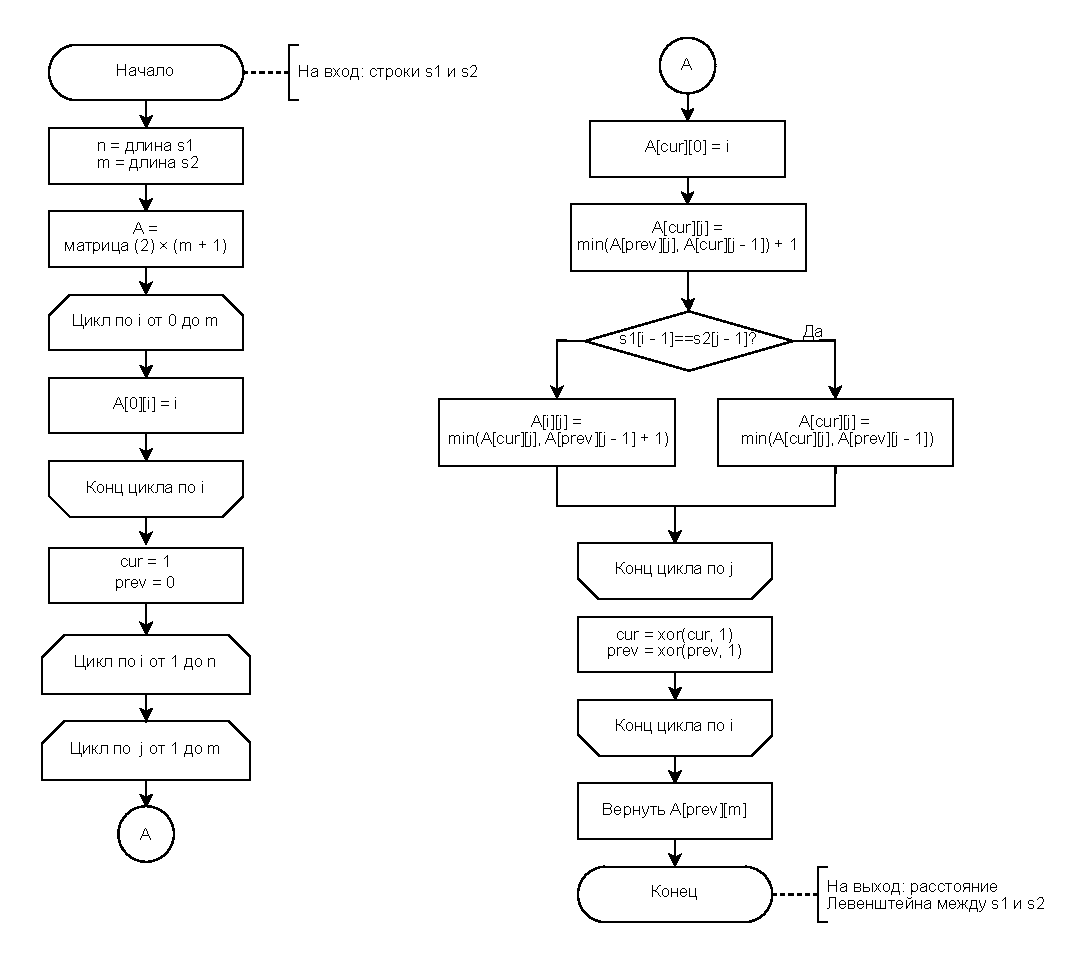
\includegraphics[width=0.8\textwidth]{lev_iter.pdf}
	\caption{Схема нерекурсивной реализации алгоритма поиска расстояния Левенштейна}
	\label{fig:lev_iter}
\end{figure}
\section{Поиск расстояния Дамерау---Левенштейна}
На рисунке~\ref{fig:dam_lev_iter} приведена схема итеративной реализации алгоритма поиска расстояния Дамерау-Левенштейна.
\subsection{Нерекурсивная реализация}
\begin{figure}[H]
	\centering
	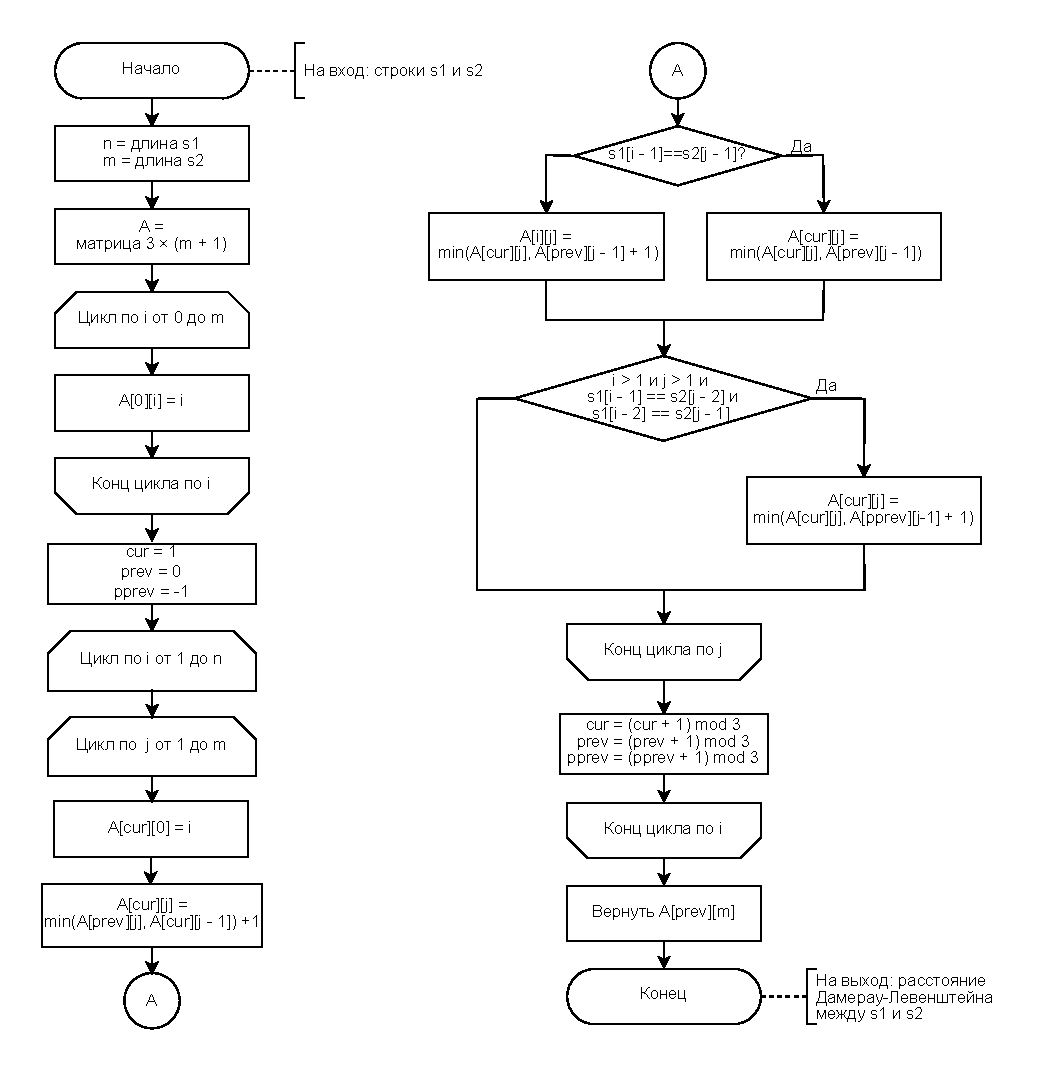
\includegraphics[width=0.8\textwidth]{dam_lev_iter.pdf}
	\caption{Схема нерекурсивной реализации алгоритма поиска расстояния Дамерау-Левенштейна}
	\label{fig:dam_lev_iter}
\end{figure}
\section*{Вывод}

На основе аналитической части построены схемы алгоритмов для реализации.

\clearpage